%!TEX root = Projektdokumentation_ClockPendulumAnalyzer.tex
\section{Projektrahmenplan}
    In diesem Kapitel werden die Meilensteine und Eckdaten wie Start- und Endzeitpunkt des Projekts festgehalten. In der Abbildung \ref{fig:rahmenplan} ist die Übersicht auf die geplanten Sprints und Meilensteine (MS) zu sehen. Die Meilensteine sowie Abgabetermine sind weiter unten in der Tabelle \ref{tab:meilensteine} ausführlicher beschrieben. Eine detaillierte Planung der jeweiligen Sprints und deren Review ist dem Anhang zu entnehmen.
    \begin{figure}[H]
        \centering
        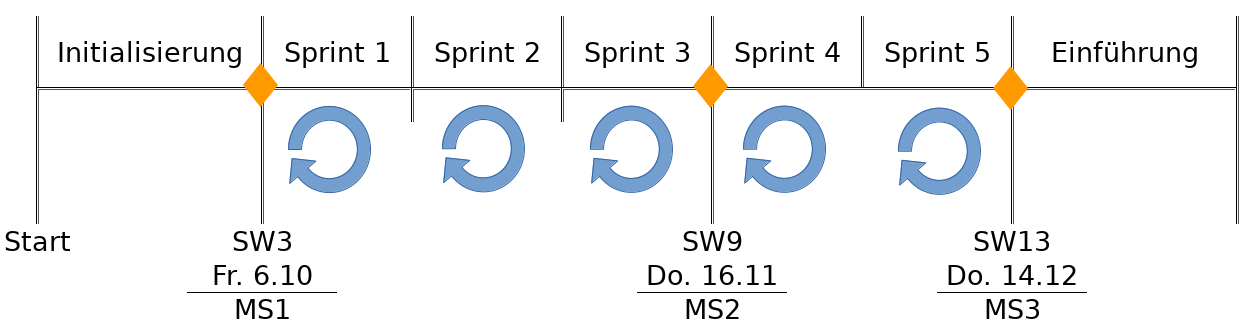
\includegraphics[width=\textwidth]{rahmenplan.png}
        \caption{Rahmenplan mit Phasen, Meilensteine und Sprints}
        \label{fig:rahmenplan}
    \end{figure}
    \begin{table}[h]
        \begin{tabularx}{\textwidth}{lll}
            \textbf{MS1:} & Zeitpunkt: & Freitag 6.10.\\
            & Artefakte: & \tabitem Projekt Management Plan (PMP)\\
            & & \tabitem Entwurf des Grobkonzepts\\
            & Ergebnisse: & \tabitem definierte Vorgehensart\\
            & & \tabitem Rahmenplanung\\
            & & \tabitem Vision (Scope, Ziele etc) im Grobkonzept\\
            \textbf{MS2:} & Zeitpunkt: & Donnerstag 16.11.2017\\
            & Artefakte & \tabitem Prototyp 1\\
            & Ergebnisse: & \tabitem lauffähiger 1. Prototyp\\
            & & \tabitem 80\% der Sys Spec\\
            \textbf{MS3:} & Zeitpunkt: & Donnerstag 14.12.2017\\
            & Artefakte & \tabitem PMP \\
            & & \tabitem SysSpec \\
            & & \tabitem Arbeitsjournal \\
            & & \tabitem Prototyp 2\\
            & Ergebnisse: & \tabitem lauffähiger 2. Prototyp\\
            & & \tabitem fertige System Spezifikation (Projektreport)\\
            & & \tabitem fertiger PMP\\
            \textbf{weitere Termine:} & & \\
            & Abgabe Dokumentation: & 05.01.2018\\
            & Abgabe Projekt: & 12.01.2018\\
            & Präsentation Projekt: & 12.01.2018\\
        \end{tabularx}
        \caption{Meilensteine und Termine}
        \label{tab:meilensteine}
    \end{table}
    